\section{Эллипс}
\begin{wrapfigure}{r}{0pt}\noindent
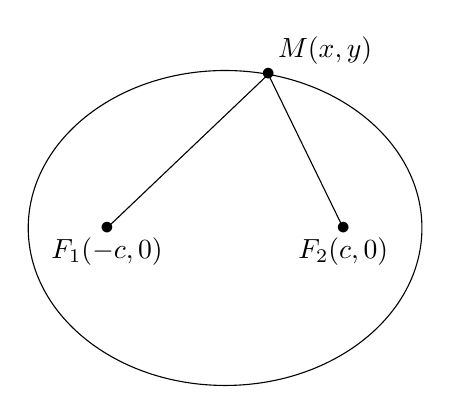
\begin{tikzpicture}[scale=0.5]
\drawaxis{-6}{6}{-5}{5};

% рисуем эллипс x^2/25 + y^2/16 = 1
\draw (-3, 0) coordinate (F1) node {$\bullet$} node[below] {$F_1(-c, 0)$}
	(3, 0) coordinate (F2) node {$\bullet$} node[below] {$F_2(c, 0)$}
	(45/41, 160/41) coordinate (M) node {$\bullet$} node [above right] {$M(x, y)$}
	-- (F1) (M) -- (F2)
	(0, 0) circle[x radius=5, y radius=4];
\end{tikzpicture}
\end{wrapfigure}

\index{Эллипс} \textbf{Эллипсом} называется геометрическое место точек~$M$ таких, что $MF_1 + MF_2 = 2a > F_1 F_2$, где $a$~--- константа, $F_1$ и $F_2$~--- фиксированные точки, называемые \textbf{фокусами эллипса}.

Пусть $F_1 = (-c, 0)$, $F_2 = (c, 0)$, $M = (x, y)$.
Найдём уравнение эллипса.
\begin{equation*}
\sqrt{(x + c)^2 + y^2} + \sqrt{(x - c)^2 + y^2} = 2a \Rightarrow
\end{equation*}
\begin{equation*}
\Rightarrow 2x^2 + 2y^2 + 2c^2 + 2\sqrt{(x^2 + y^2 + c^2)^2 - 4c^2 x^2} = 4a^2 \Rightarrow
\end{equation*}
\begin{equation*}
\Rightarrow (2a^2 - (x^2 + y^2 + c^2))^2 = (x^2 + y^2 + c^2)^2 - 4c^2 x^2 \Leftrightarrow
\end{equation*}
\begin{equation*}
\Leftrightarrow a^4 - a^2 x^2 - a^2 y^2 - a^2 c^2`+ c^2 x^2 = 0 \Leftrightarrow
\end{equation*}
\begin{equation*}
\Leftrightarrow (a^2 - c^2) x^2 + a^2 y^2 = a^2 (a^2 - c^2) \Leftrightarrow
\end{equation*}
\begin{equation*}
\left|\text{Пусть $b^2 = a^2 - c^2$}\right|
\Leftrightarrow b^2 x^2 + a^2 y^2 = a^2 b^2 \Leftrightarrow
\frac{x^2}{a^2} + \frac{y^2}{b^2} = 1
\end{equation*}

\subsection{Уравнение касательной}
Найдём уравнение касательной, проходящей через точку~$(x_0, y_0)$ эллипса.
\begin{equation*}
y = \pm b\,\sqrt{1 - \frac{x^2}{a^2}} \Rightarrow
y' = \pm\frac{ab}{2\sqrt{a^2 - x^2}} \cdot \frac{-2x}{a^2} =
\mp\frac{bx}{a\sqrt{a^2 - x^2}} \;
\left|y = \pm b\,\sqrt{1 - \frac{x^2}{a^2}} \Leftrightarrow
\sqrt{a^2 - x^2} = \pm\frac{a}b\,y\right| =
-\frac{b^2 x}{a^2 y}
\end{equation*}
\begin{equation*}
y = y_0 - \frac{b^2 x_0}{a^2 y_0} (x - x_0) \Leftrightarrow
a^2 (y - y_0) y_0 = -b^2 (x - x_0) x_0 \Leftrightarrow
\frac{x x_0}{a^2} + \frac{y y_0}{b^2} - \left(\frac{x_0^2}{a^2} + \frac{y_0^2}{b^2} \right) = 0 \Leftrightarrow
\frac{x x_0}{a^2} + \frac{y y_0}{b^2} = 0
\end{equation*}